%%%%%%%%%%%%%%%%%%%%%%%%%%%%%%%%%%%%%%%%%%%%%%%%%%%%%%%%%%%%%%%%%%%%%%%%%%%%%%%%
% Author : Jan Lipensky, Tomas Polasek (template)
% Description : Seventh exercise in the Introduction to Game Development course.
%   It deals with the creation of a Game Design Document, presenting a short 
%   pitch for a potential game project.
%%%%%%%%%%%%%%%%%%%%%%%%%%%%%%%%%%%%%%%%%%%%%%%%%%%%%%%%%%%%%%%%%%%%%%%%%%%%%%%%

\documentclass[a4paper,10pt,english]{article}

\usepackage[left=2.50cm,right=2.50cm,top=1.50cm,bottom=2.50cm]{geometry}
\usepackage[utf8]{inputenc}

% Hyper-Text References
\usepackage{hyperref}
\hypersetup{colorlinks=true, urlcolor=blue}

% Drawing Images and Graphs
\usepackage{tikz}
\usepackage{pgfplots}

% Page Utilities
\usepackage{graphicx}

% Image Sub-Captions
\usepackage{subcaption}

\newcommand{\ph}[1]{\textit{[#1]}}

\title{%
Game Pitch Document%
}
\author{%
Jan Lipenský (xlipen02)%
}
\date{}

\begin{document}

\maketitle
\thispagestyle{empty}

{%
\large

\begin{itemize}

\item[] \textbf{Title:} The Game

\item[] \textbf{Genre:} VR Real-life RPG

\item[] \textbf{Style:} 3D VR Realistic

\item[] \textbf{Platform:} PC, PS5

\item[] \textbf{Market:} Immersive gaming enthusiasts, 18+

\item[] \textbf{Elevator Pitch:} Bored with reality? Join us for a thrilling adventure and start anew!

\end{itemize}

}

\section*{\centering The Pitch}


\subsection*{Introduction}
What if \emph{The Sims} and \emph{GTA} had a baby? \emph{The Game} would be born! A VR Experience like no other. In our game, you could do everything you have ever dreamt of. Afraid of asking for that raise? Afraid of asking that person on a date? In \emph{The Game}, there is no need to be scared! 


\subsection*{Background}
The idea for this game was to create a truly unique gaming experience. \emph{The Game} would be the biggest game to date. If you ever thought that \emph{The Sims} was too cartoonish and restrictive, while \emph{GTA} never really focused on character building, this game will be perfect for you. Here you can build your life from the ground up. Experience school like never before. Relive the joy of getting your first job and buying your first car, but better! But... if you are not into this, you can also be a GTA-style criminal! Everything is possible here, there are practically no limits!

\subsection*{Setting}
The game will be set in a carefully crafted replica of our Earth. We have done investigative road trips across the globe to really try to capture the world 1:1. At the start, you will have to choose your family background and a short story based on your choice will play out. The protagonist (\emph{you}) can be created to any liking you want him to be. You can also choose the starting age. The earliest is 18 years old. Choosing your family background will greatly impact your early game (financial status of your family, relationships, ...), and every background has special quests, which are not mandatory to complete. The game won't hold your hand, you are completely free.

\subsection*{Features}

\begin{itemize}
\item \textbf{Life Unleashed:} Experience one-of-a-kind freedom as you live out your life in a realistic 3D world that mirrors our own. Shape your life from adolescence to old age with nearly limitless possibilities at your disposal.

\item \textbf{Your own Storytelling:} Choose your family background, create unique relationships, and do quests tailored to your character's origin. Every decision you make influences your virtual life, providing a truly personalized narrative.

\item \textbf{Open-World Realism:} Experience a perfectly crafted replica of Earth, with locations you love. Explore our world with the best attention to detail to date.

\item \textbf{You are The Protagonist:} Create a character that reflects your identity, or play as someone completely different. From education and career choices to relationships and hobbies, your only limit is the sky!

\item \textbf{Limitless Possibilities:} If you want to have a successful job, that you would love, or if you want to experience the thrill of a criminal life, the choice is yours. \emph{The Game} offers a vast array of activities, ensuring there's something for every player. But remember, your actions might have big consequences! 

\item \textbf{Realistic Simulation:} Blending the best elements of \emph{The Sims} and \emph{GTA} offers a one-of-a-kind game of life simulation and open-world action. From basic tasks to high-stakes heists, everything is designed for maximum realism. You also have to maintain yourself! Drink, eat, go to the gym... And shower once in a while!

\item \textbf{Immersive VR Experience:} Experience virtual reality world that transcends traditional gaming. \emph{The Game} features cutting-edge VR technology for a truly immersive gaming adventure.

\item \textbf{Endless Replayability:} With almost limitless choices, storylines, and an evolving world, each playthrough offers a fresh and unpredictable experience. \emph{The Game} makes sure that no two journeys are alike.
\end{itemize}


\begin{figure}[h]

\centering
    
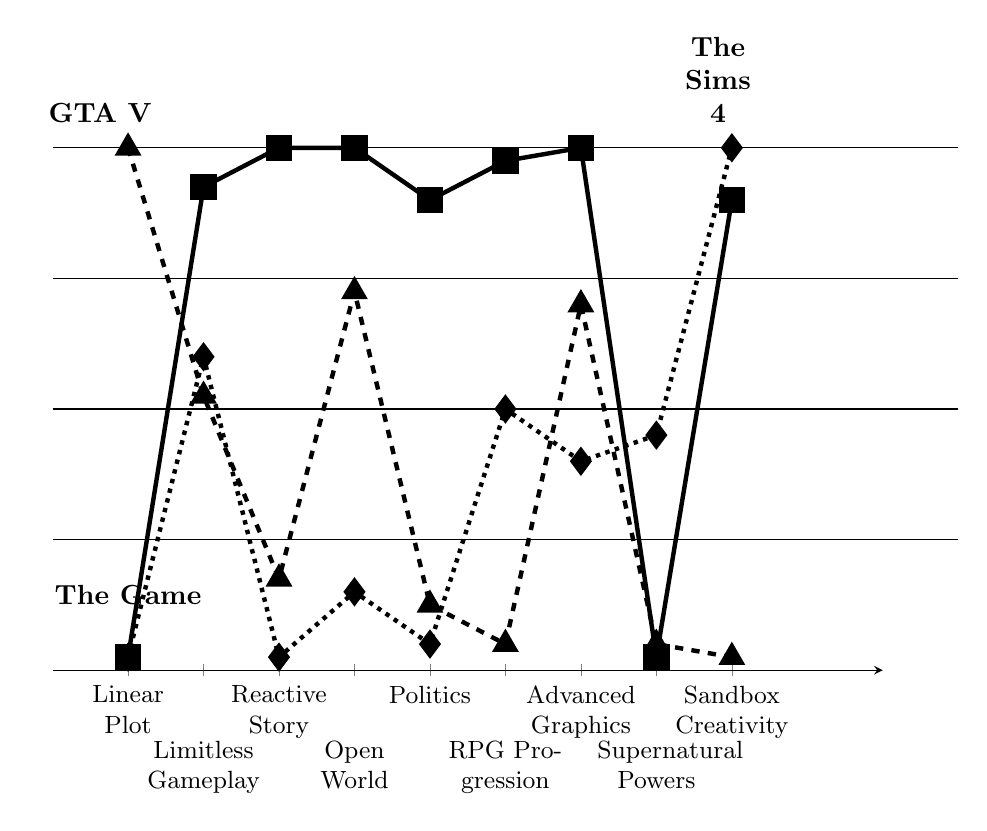
\begin{tikzpicture}[remember picture]%
\begin{axis}[
    domain=0:1, 
    clip=false, 
    ymin=0, xmin=0, ymax=4.1, xmax=11, 
    xtick={1,2,...,9}, 
    yticklabels={}, 
    xticklabels={Linear Plot, Limitless Gameplay, Reactive Story, Open World, Politics, RPG Progression, Advanced Graphics, Supernatural Powers, Sandbox Creativity}, 
    xticklabel style={yshift={-mod(\ticknum, 2) * 2em}, text width=1.5cm, font=\small, align=center}, 
    y tick style={draw=none}, 
    x axis line style={|-|}, 
    y axis line style={draw=none}, 
    axis lines=middle, 
    width=1\linewidth, 
    height=0.3\paperheight
]
    \addplot [ultra thick, mark=square*, mark options={scale=2,solid}] coordinates {
        (1, 0.1)
        (2, 3.7)
        (3, 4)
        (4, 4.0)
        (5, 3.6)
        (6, 3.9)
        (7, 4)
        (8, 0.1)
        (9, 3.6)
    } node[above, yshift=15pt, pos=0] {\textbf{The Game}};
    
    \addplot [ultra thick, dashed, mark=triangle*, mark options={scale=2,solid}] coordinates {
        (1, 4)
        (2, 2.1)
        (3, 0.7)
        (4, 2.9)
        (5, 0.5)
        (6, 0.2)
        (7, 2.8)
        (8, 0.2)
        (9, 0.1)
    } node[above, yshift=5pt, xshift=-10pt, pos=0] {\textbf{GTA V}};
    
    \addplot [ultra thick, dotted, mark=diamond*, mark options={scale=2,solid}] coordinates {
        (1, 0.1)
        (2, 2.4)
        (3, 0.1)
        (4, 0.6)
        (5, 0.2)
        (6, 2)
        (7, 1.6)
        (8, 1.8)
        (9, 4)
    } node[above, yshift=5pt, xshift=-5pt, pos=1, text width=1cm, align=center] {\textbf{The Sims 4}};
    
	\draw [] (axis cs:{0,1}) -- (axis cs:{12,1});
	\draw [] (axis cs:{0,2}) -- (axis cs:{12,2});
	\draw [] (axis cs:{0,3}) -- (axis cs:{12,3});
	\draw [] (axis cs:{0,4}) -- (axis cs:{12,4});
\end{axis}
\end{tikzpicture}


\caption{Value graph for \emph{GTA V}, \emph{The Game}, and \emph{The Sims 4}.}
\label{Fig:ValueGraph}

\end{figure}

\subsection*{Genre}
The game will mainly focus on the life-building aspect while maintaining a strong RPG connection. We cannot summarize \emph{The Game} in genres, since we believe our game will create a whole new genre and revolutionize gaming! But we believe our core genres are these:
\begin{itemize}
    \item \textbf{Social simulation}
    \item \textbf{Realistic RPG}
    \item \textbf{Sandbox RPG}
    \item \textbf{Action Game}
\end{itemize}
The genre of the game really depends on your playstyle though!
\subsection*{Platform}
\emph{The Game} will be released on \emph{Windows PC} and the \emph{Playstation 5} console, since no other platform currently supports VR in a way that would technologically allow \emph{The Game} to exist and be playable.

\subsection*{Style}
The game will feature hyper-realistic graphics. Our graphic artists are working hard to make it look like our real world, so the players can feel more immersed and enjoy the game. Below, are some concept arts by our Graphics Design team.

\begin{figure}[h]

\centering

\begin{subfigure}{0.29\linewidth}
\includegraphics[width=\linewidth]{figA}
\captionof{figure}{Work 1a.}
\label{Fig:Style1A}
\end{subfigure}\hfill
%
\begin{subfigure}{0.29\linewidth}
\includegraphics[width=\linewidth]{figB}
\captionof{figure}{Police Investigation 1b.}
\label{Fig:Style1B}
\end{subfigure}\hfill
%
\begin{subfigure}{0.29\linewidth}
\includegraphics[width=\linewidth]{figC}
\captionof{figure}{Relationships 1c.}
\label{Fig:Style1C}
\end{subfigure}

\end{figure}


\end{document}
